\section{On segmentation and single-cell features}
\label{imaging:features}


Once a dataset has been collected, and corrected as
in the previous section, the analysis begins. In general,
we want to obtain interesting properties of the foreground
layers in our images. In specific, it is nearly always the
foreground properties within individual cells that we care
about. ``Segmentation'' is the process of identifying
those cells (or intracellular objects)
and extracting them from the rest of the image.
Once cells have been segmented, properties of their pixel
values and spatial arrangement can be measured and stored
as sets of features.


Cellular segmentation is still an unsolved computer
vision problem \cite{Danuser2011},
in large part because experimental needs are too specific
to allow for a good general solution. There is, however,
an array of partial solutions available. These range from simple
to highly complex, and vary tremendously in their accuracy
and utility.
In this section I briefly discuss segmentation algorithms
and how one can go about choosing single-cell
features that are biologically meaningful.
My goal in part is to provide
the rationale for my own choices for the
experimental work in \ar{insulation:introduction}.


\subsection{Segmentation approaches}
\label{imaging:segmentation}

There are many approaches to cellular segmentation.
Software solutions such as CellProfiler \cite{Carpenter2006}
implement many of the most-used segmentation algorithms
so that the user can choose one appropriate to the experiment.
Unfortunately, which algorithm should be chosen is not a trivial matter.
Many of these algorithms are complex and therefore difficult
to understand and use. Further, the simpler algorithms may fail
to provide sufficiently accurate segmentation for some image properties.
As a consequence the path of least resistance is often manual segmentation
using tools such as ImageJ \cite{Schneider2012},
but this labor-intensive approach limits the resulting sample
size and may yield biased investigator-specific outcomes.


The value of automated segmentation approaches should be obvious:
they allow for the rapid and reproducible
identification of huge numbers of cells. Automated approaches are
also biased, due to the choice of parameters for the algorithm, but
the bias is systematic and does not change between images.
There are plenty of difficulties with automation, however. With
huge datasets comes the inability to perform thorough quality
control. Additonally, there may be no single set of segmentation parameters,
or even a single algorithm, that will successfully segment all
cellular phenotypes in a diverse experimental setup (e.g. a
drug screen). Automation thus requires extensive testing and
a wary mindset.


As a consequence of these issues, I strongly advocate for use of the simplest
segmentation method that is capable of answer a given
experimental question. Because so many aspects of images
can be measured, it is easy to get carried away with trying to
obtain every single piece of data that the images contain. As already noted, however,
the number of potential measurements is large;
obtaining all data from images is not only impossible, it probably
is not wise since each extracted feature should be understood at a
biological level before it is used (and, as I discuss below, biological
interpretation of features is not a trivial task).
The use of simpler methods makes the resulting segmentation more 
understandable, and so conditions that will cause the algorithm
to produce garbage are more predictable and intuitive. A few of
the more straight-forward and commonly-used methods are
threshold, watershed, and voronoi segmentation, discussed next
(these are depicted graphically in \ar{fig:imaging:segmentationMethods}).


  \begin{figure}[!bt]
  \centering
  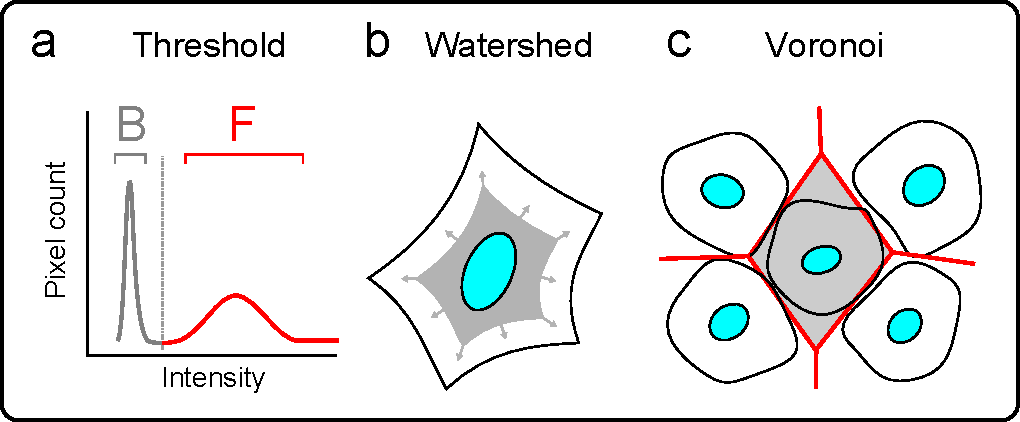
\includegraphics[width=4in]{FIGS/imaging/segmentationMethods.pdf}
  {\singlespacing 
  \caption[ Cartoon of segmentation methods.]
            {Cartoons of three basic segmentation
            methods. \b{a}, Threshold segmentation separates
            background $B$ from foreground $F$ by fluorescence
            intensity. Neighboring pixels are then considered
            part of the same object. The histogram
            represents the distribution of
            all pixel intensities within an image.
            \b{b}, Watershed starts with a known
            intracellular point (e.g. the nucleus, blue)
            and moves outwards (gray, arrows) until it reaches
            cell boundaries. \b{c} Voronoi segmentation assigns
            to a set of already-known objects all of the space closer to
            that object than any other. Red lines, boundaries
            of the Voronoi cells,
            using nuclei centroids as the known points. Gray area,
            segmented region for the middle cell.}
  \label{fig:imaging:segmentationMethods}}
  \end{figure}
  
  
Threshold segmentation (the approach that I use in this
dissertation) is probably the simplest method after manual
segmentation. It works by assuming that the pixel intensities
within cells are generally higher then those in the image
background \ar{fig:imaging:segmentationMethods}a.
Therefore a threshold can be chosen either manually
or via some mathematical or algorithmic approach (e.g.
Otsu thresholding \cite{Otsu1975}) that best separates
background and foreground pixels. Neighboring pixels classified
as foreground can be grouped into
objects, such as nuclei. This method tends to fail for whole-cell
segmentation when
cellular density is high, as neighboring cells can be segmented
as single objects. Additionally, it is not necessarily true
that the nuclear or cytosolic compartments contain higher
pixel intensities than do the background. This is dependent
on the probes used, and is of particular difficulty for
live-cell imaging (see Appendix \ar{pseg} for an experimental solution).
Cellular nuclei are frequently
segmented using this method, as they tend to be spatially distinct
even with high cell density, and DNA stains such as Hoechst
and DAPI create bright foreground signals. Threshold-segmented
nuclei often form the basis for more complex algorithms.


There are many specific algorithms for watershed segmentation
\cite{Vincent1991,Malpica1997,Loo2010} but the general
approach is roughly the same. The algorithm starts with
a ``seed,'' which is a pixel coordinate in the image.
This seed can be randomly generated or chosen from centroids
of threshold-segmented nuclei. The algorithm then searches
away from that seed point, following paths of increasing
intensity (\ar{fig:imaging:segmentationMethods}b).
Sharp decreases in intensity, as frequently
occurs between cells or between a cell edge and the background,
will cause the outward movement to stop. These algorithms
are thus useful for segmenting irregularly-shaped and slightly
crowded cytosolic regions. However, they may require many parameters, and
can yield over-segmentation (the breaking up of single cells
into many objects).


The final method that I want to make note of is Voronoi
segmentation. I have not frequently seen this method used in
the context of segmenting cells in tissue culture, but it
can be useful in the case that cells are at an extremely
high density (so that there is no background) and when
those cells are similar in size and relatively round
or cuboidal. With this approach,
a set of seeds are again needed. These will typically be
the centroids of threshold-segmented nuclei. For each centroid,
then, the algorithm assigns to it all space closer to that centroid
than to any other (\ar{fig:imaging:segmentationMethods}c).
This is a simple and efficient method for roughly segmenting
cellular cytosolic compartments.


With this brief overview of few segmentation methods, a
few points should be clear. First, many segmentation
approaches are fluorescence-based (though some use
brightfield) and so require staining of the cellular
compartments to be segmented (see Appendix \ar{pseg} for a live-cell
solution to this). Second, nuclei are much simpler
to segment than cytosolic regions, because nuclei typically
have narrower ranges of size, shape, and staining intensity.
Therefore threshold segmentation of
nuclei is generally considered to be accurate, and is
a frequent first-step for more complicated segmentation
pipelines. Third, different foreground objects may
require different algorithms for accurate segmentation.
Taken together, the above points help to explain why cellular
segmentation does not have a general solution.



\subsection{Understanding and choosing single-cell features}

Given the nearly unlimited set of features to choose from
it can be difficult to determine the subset that is most
appropriate to the study at hand. There are a few broad
approaches to this problem. The obvious, but non-trivial, approach is to
first choose the biological property of interest and then
identify or create features that approximate that property.
A less obvious approach is to obtain a large number of
features and use computational methods to choose those that
are the most informative \cite{Singh2010}.
In the latter case, the features need
not be biologically interpretable at all. For this discussion
I focus on the first case.


Biologically-motivated features are necessarily approximations
of the underlying property of interest. It is therefore important
to be aware of how the features are defined so that the data
can be interpreted properly. As an example, a project in the
Altschuler \& Wu lab required measurement of neutrophil polarity, but
needed that measurement to be performed on fluorescently-labeled
cytoskeletal components. There is no obvious mathematical
feature of fluorescently-labeled actin or microtubules that would indicate the
degree of polarization of a neutrophil. An approximate solution was
therefore developed, which measures how close together in space are the brightest
pixels \cite{Ku2010,Ku2012}.


This polarity feature will decrease in value with, for example, 
increased collection of actin to one side of the cell.
In the case that the actin intensity is diffuse throughout
the cell, the brightest pixels will also be
diffuse and so the feature value increases.
This feature therefore serves as a useful proxy for polarity. However,
the feature is sensitive to bright punctate artifacts that
are common to immunostained images and is distorted by differences in
cell size. By being aware of these pitfalls they can
be addressed. In this case, visual quality control was performed
on every cell to ensure
the absence of artifacts, and the feature calculation was modified to compensate
for distortions due to cell size \cite{Ku2010,Ku2012}.


Investigators will more frequently use combinations of
simpler features, such as those describing aspects of cell
size and shape (``morphological features'') and
of fluorescence intensity (``intensity features''). It is
important to be aware that these two classes are not completely
independennt. Intensity features in particular can be highly
dependent on morphological features.


As a simple example,
the average intensity is dependent on the area.
It is therefore important to interpret changes to the average
with care, as the change could result from  a
change in cell size, a change in concentration of the labeled
protein, or a combination of the two.
The ratio of nuclear to cytosolic average intensities
additionally suffers from this potential confusion. It has
an added difficulty, however, in that a change in the ratio
can be due to movement of the labeled protein from one compartment
to the other, or to independent changes in one or both compartments.


Ideally, then, a
feature should be carefully chosen to have an unambiguous biological
interpretation and be independent of
other features whose changes are not important to
the study. I argue that interpretability is more important than having
a feature that more closely approximates the biological property
of interest. For example, in my own work (\ar{insulation:introduction})
I am interested in the
concentrations of nuclear transcription factors. Concentration
is intuitively approximated by the average intensity feature, yet
I instead chose the total intensity feature for all of my analysis.
I did so because certain properties of the total intensity feature,
discussed next, allow for less ambiguity in how to interpret
changes in its values.


\subsection{Benefits of the total nuclear intensity feature}
\label{imaging:totalIntensity}


The total intensity
feature is a proxy for the absolute count
of a fluorescently-labeled target molecule. This feature has the
advantage of being independent of cell size, such that changes
in cell morphology may change the average but not total
intensity. Unfortunately, intensity from widefield microscopy images
does not just come from the focal plane, but also from the
space both above and below that plane. As a consequence,
in image represents a messy volumetric cross section through the $z$-axis.
This fact adds some complication to the interpretation of the
total intensity feature: is it measuring the total number of
molecules in the entire cell volume, from a thin cross-section,
or something in between?


Fortunately, my focus on transcription factors in 
\ar{insulation:introduction} allows me to mitigate this concern
by measuring only the nuclear intensities. The nucleus
tends to maintain a taller stature in the $z$-axis than does
the rest of the cell (resulting in the famous ``fried egg'' appearance
of cells in tissue culture). Also, nuclei tend to be of
more similar size and shape than do cytosolic compartments.
For these reasons, I can reasonably assume that whatever the
thickness of the imaged section, I will be imaging a similar
thickness for all nuclei.


Finally, and perhaps most importantly, the nucleus
has a built-in ``ground truth'' for this feature that allows
for both quality control and removal of measurement error
\arp{imaging:variation}.
This ground truth comes from the DNA content of cells, as
each cell within e.g. the G1 phase of the cell cycle in reality
has a near-identical total DNA content. The total intensity
feature is a proxy for this content. Importantly,
total nuclear intensity is the only feature
with such a ``ground truth'' reference.
The small-molecule stain Hoechst
provides a robust and DNA-specific signal that I use throughout
this dissertation to measure total DNA content. I therefore use
the term ``DNA'' interchangeably to refer to the actual molecule
and as a short-hand for ``Hoechst-stained DNA.'' 


\subsection{Measuring information content of a feature}
\label{imaging:information}

One of the major hurdles in experimental cell biology
is our lack of initial knowledge about which environmental
signals ($S$) and cellular responses ($R$) cells care about
(discussed in \ar{introduction:introduction}).
As a consequence, it is generally unclear how
much information about the environment a cell can accurately process
and store, though estimates suggest that the features
we believe cells care about contain
somewhat unimpressive information content \cite{Cheong2011}.

  \begin{figure}[!bt]
  \centering
  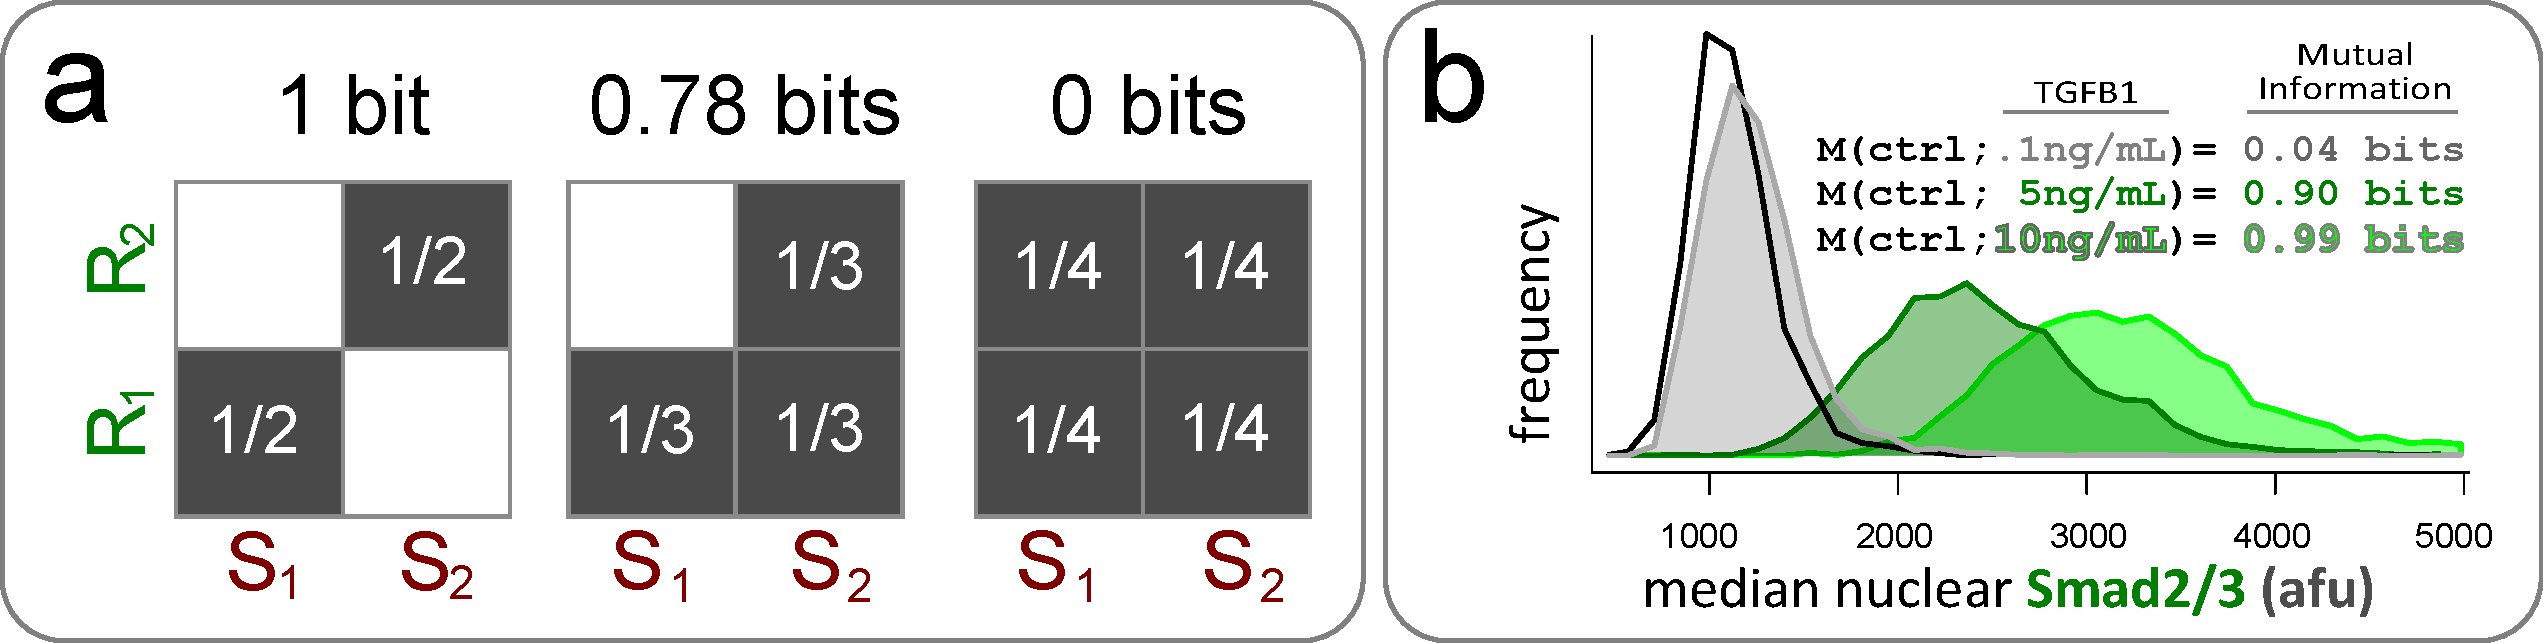
\includegraphics[width=6in]{FIGS/imaging/MI.pdf}
  {\singlespacing 
  \caption[ Mutual information examples.]
            {The mutual information metric can be interpreted
            as yielding $\log_2$ of the number of distinct signal-response
            relationships. \b{a}, A toy cases with
            only two signals, $S_1$ and $S_2$, and two responses,
            $R_1$ and $R_2$, with uniform joint probabilities. Darkened
            boxes show occurring signal-response relationships and their
            joint probabilities. Left, two completely distinct
            signal-response pairs yield $\log_2(2)=1$ bit of mutual
            information. Middle, both signals cause response $R_1$,
            meaning that observation of $R_1$ provides insufficient
            information to know which signal caused that response. The mutual
            information thus decreases to $\log_2(81/16)\approx0.78$
            bits (using \ar{eq:imaging:mi}). Right, with both signals
            causing both responses with equal probability, there is
            no mutual information ($\log_2(1)=0$ bits).
            \b{b}, Mutual information measurements of TGFB1-Smad2/3
            responses. Distributions show the wide variability
            of nuclear Smad2/3 accumulation even in response to
            saturating (10ng/mL) ligand concentrations. Observe
            that the control and saturating doses yield distributions
            that are nearly non-overlapping, and as a consequence
            yield $\sim$1 bit of mutual information (as there are 2
            distinct signal-response relatinships). It should be clear
            that the mutual information between all concentrations and
            outputs can be calculated at once, but there is significant
            overlap between all but the outermost distributions. Thus,
            addition of each subsequent intervening signal will in this
            case yield diminishing improvements to the mutual information
            between TGFB1 and nuclear Smad2/3.
            $n$>3000
            human colonic epithelial cells per condition. I used
            an implementation of the mutual information algorithm as described
            in \cite{Cheong2011}.}
  \label{fig:imaging:MI}}
  \end{figure}

Measuring the information content of a feature with
respect to the signal under study can therefore be useful
when trying to choose between a set of potential $(S,R)$
combinations. This can be
done using the ``mutual information'' metric
between the signal and response, $M(S;R)$  \cite{Cheong2011}.
Mutual information has advantages over other statistical metrics,
such as Z-scores and the like, in that it is completely
non-parametric (i.e. does not assume a distribution shape)
and uses units that
can be directly interpreted as ``information content,'' measured in bits.
I use this metric in \ar{insulation:introduction} to compare
the information content of ligand concentrations for \tgfbsf\
and Wnt, and so here I dig into mutual information a bit
deeper\footnote{Did you catch the joke?}
with the goal of providing an intuition to the reader
regarding its interpretation.


The mutual information between a set of signals $S$
(e.g. ligand concentrations) and
responses $R$ (e.g. nuclear transcription factor concentrations) is defined
by \ar{eq:imaging:mi}. In the formula, $P(R,S)$ is the joint
probability of each signal-response pair
and $P(R)$ and $P(S)$ are the marginal
probabilities.
The mutual information value returned by this formula
is in units of ``bits,'' and can
be interpreted as the $\log_2$ of the number of
distinct signal-response relationships
(see \ar{fig:imaging:MI}a for a toy example).
In essence the quantity describes how accurately
we would be able to guess the signal if we were
told the response (and vice versa).
The goal of the mutual information metric then
is to measure the degree of overlap between
signal-response distributions, it is not to measure
how far apart those distributions are. For example,
two completely separated response distributions will
always have 1 bit of mutual information even if they
are infinitely far apart. Therefore the maximum possible
information content is $\log_2$ of the number of distinct
signals (\ar{fig:imaging:MI}a, left). The minimum mutual information is zero, which
occurs when the distributions completely overlap (\ar{fig:imaging:MI}a, right).
    %
    \begin{equation} \label{eq:imaging:mi}
    M(R;S)=\sum_S\sum_R P(R,S)\log_2\left(\frac{P(R,S)}{P(R)P(S)}\right)
    \end{equation}



Importantly, single-cell
variability in nuclear transcription factor
concentrations is high, such that even the
untreated and saturating ligand
doses yield a small overlap in cellular
responses (\ar{fig:imaging:MI}b) \cite{Cheong2011}. In other words,
if we were given a randomly drawn cellular Smad2/3
response from a dose-response curve for TGFB1 treatment,
we would have high uncertainty as to the precise
TGFB1 concentration that caused the drawn response.


In summary, mutual information is a metric that
measures the overlap of distributions, and so can
be interpreted to indicate the number of distinct
signal-response pairs for a given feature. This
metric can thus be used to directly measure the
relative information content of different features $R$
or signals $S$ (as I do in \ar{insulation:system}).